\documentclass{article}
\usepackage[paperwidth=5.5cm,paperheight=5.3cm,left=0cm,right=0cm,bottom=0cm,top=0.25cm]{geometry}
\usepackage{tikz}
\definecolor{fom}{RGB}{0,153,139}
\begin{document}
 
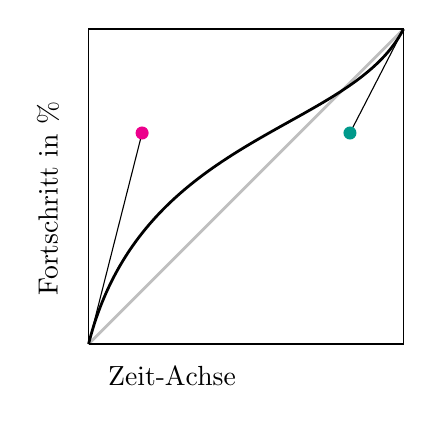
\begin{tikzpicture}[x=4cm,y=4cm]
\draw[line width=1pt,lightgray] (0,0) -- (1,1); % gray line for the linear animation path
\draw (0,0) -- (1,0) -- (1,1) -- (0,1) -- (0,0); % frame
\draw (0,0) -- (0.17,0.67); % (0,0) to 2. point
\draw (1,1) -- (0.83,0.67); % (1,1) to 3. point
 
\draw [magenta,fill=magenta](0.17,0.67) circle (.5ex); %circle 1
\draw [fom,fill=fom](0.83,0.67) circle (.5ex); % circle 2
 
\draw[line width=1pt] (0,0) .. controls (0.17,0.67) and (0.83,0.67) .. (1,1); % cubic bezier curve
 
% labels
\node[label={[label distance=0.0cm,text depth=-1ex,rotate=90]left:Fortschritt in \%}] at (-0.1,.8) {};
\node[label={[label distance=0.0cm,text depth=-1ex]right:Zeit-Achse}] at (0,-0.1) {};
\end{tikzpicture}
\end{document}